\section{Módulo JavaScript EmberJS}

O \textit{frontend} do subsistema, módulo responsável pela visualização dos
dados, tinha como resultados esperados uma aplicação que pudesse prover a
visualização dos sinais referentes a um determinado paciente, baseado nas
informações recebidas do servidor de \textit{backend}. Devido à necessidade de
uma certa dinamicidade na apresentação destes dados, foi escolhido o
\textit{Framework JavaScript EmberJS \footnote{\url{https://emberjs.com/}}}.

Desta forma, foi então desenvolvida a aplicação
UMISS-frontend\footnote{\url{https://github.com/cadeiracuidadora/UMISS-frontend}},
que apresenta de forma gráfica e textual o histórico dos sinais monitorados pelo
projeto UMISS.

Baseado no \textit{token} fornecido em cada cadeira, o usuário monitor pode
fazer o cadastro na aplicação e a partir de então fazer o monitoramento do
paciente vinculado à cadeira em questão. O servidor de \textit{backend} é
responsável pela filtragem dos dados recebidos, garantindo então que apenas os
dados do paciente vinculado ao token fornecido possam ser visualizados pelo
usuário monitor.

\begin{figure}
  \begin{center}
    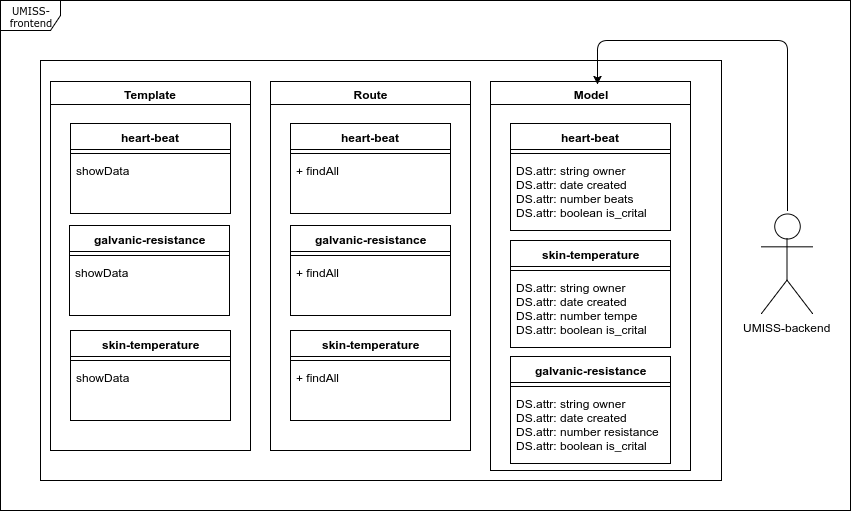
\includegraphics[scale=0.5]{figuras/frontarch.png}
  \end{center}
  \caption{Diagrama da arquitetura parcial do UMISS-frontend.}
  \label{fig:frontarch}
\end{figure}
